\documentclass[12pt,a4paper]{article}
% Some basic packages

% \usepackage[utf8]{inputenc}
% \usepackage[T1]{fontenc}
% \usepackage{textcomp}
% \usepackage[dutch]{babel}

\usepackage[T1,T2A]{fontenc}
\usepackage[utf8]{inputenc}
% \usepackage[english,russian]{babel}

% \usepackage[utf8]{inputenc}
% \usepackage[T2A]{fontenc}

\usepackage{url}
\usepackage{graphicx}
\usepackage{float}
\usepackage{booktabs}
\usepackage{enumitem}

\newcount\pdfminorversion
\pdfminorversion=7

% Don't indent paragraphs, leave some space between them
\usepackage{parskip}

% Hide page number when page is empty
\usepackage{emptypage}
\usepackage{subcaption}
\usepackage{multicol}
\usepackage{xcolor}

% page size settings
\usepackage{fullpage}
% \usepackage[top=2cm, bottom=4.5cm, left=2.5cm, right=2.5cm]{geometry}
% \usepackage[top=1cm, bottom=1.5cm, left=2cm, right=4cm]{geometry}
\usepackage[top=1cm, bottom=2cm, outer=2cm, inner=2cm, heightrounded, marginparwidth=3cm, marginparsep=1cm,headsep=0.6cm]{geometry}

% for notes at the left side
\usepackage{marginnote}

% Other font I sometimes use.
% \usepackage{cmbright}

\usepackage{hyperref}
\hypersetup{%
  colorlinks=true,
  linkcolor=blue,
  linkbordercolor={0 0 1}
}

% force display math for all environements
\everymath{\displaystyle}

\usepackage{witharrows}

% Math stuff
\usepackage{amsmath, amsfonts, mathtools, amsthm, amssymb}
% Fancy script capitals
\usepackage{mathrsfs}
\usepackage{cancel}
% Bold math
\usepackage{bm}
% Some shortcuts
\newcommand\N{\ensuremath{\mathbb{N}}}
\newcommand\R{\ensuremath{\mathbb{R}}}
\newcommand\Z{\ensuremath{\mathbb{Z}}}
\renewcommand\O{\ensuremath{\emptyset}}
\newcommand\Q{\ensuremath{\mathbb{Q}}}
% \newcommand\C{\ensuremath{\mathbb{C}}}

% Easily typeset systems of equations (French package)
\usepackage{systeme}

% Put x \to \infty below \lim
\let\svlim\lim\def\lim{\svlim\limits}

%Make implies and impliedby shorter
\let\implies\Rightarrow
\let\impliedby\Leftarrow
\let\iff\Leftrightarrow
\let\epsilon\varepsilon

% Add \contra symbol to denote contradiction
\usepackage{stmaryrd} % for \lightning
\newcommand\contra{\scalebox{1.5}{$\lightning$}}

% \let\phi\varphi

% Command for short corrections
% Usage: 1+1=\correct{3}{2}

\definecolor{correct}{HTML}{009900}
\newcommand\correct[2]{\ensuremath{\:}{\color{red}{#1}}\ensuremath{\to }{\color{correct}{#2}}\ensuremath{\:}}
\newcommand\green[1]{{\color{correct}{#1}}}

% horizontal rule
\newcommand\hr{
    \noindent\rule[0.5ex]{\linewidth}{0.5pt}
}

% hide parts
\newcommand\hide[1]{}

% % si unitx
% \usepackage{siunitx}
% \sisetup{locale = FR}

% Environments
% \makeatother
% For box around Definition, Theorem, \ldots
\usepackage{mdframed}
\mdfsetup{skipabove=1em,skipbelow=0em}
\theoremstyle{definition}
\newmdtheoremenv[nobreak=true]{characteristic}{Characteristic}
\newmdtheoremenv[nobreak=true]{lemma}{Lemma}
\newmdtheoremenv[nobreak=true]{law}{Law}
\newmdtheoremenv[nobreak=true]{postulate}{Postulate}
\newtheorem*{practical}{Practical}
\newtheorem*{terminology}{Terminology}
\newtheorem*{example}{Example}

\newmdtheoremenv[nobreak=true]{definition}{Definition}
\newtheorem*{eg}{Example}
\newtheorem*{notation}{Notation}
\newtheorem*{previouslyseen}{As previously seen}
\newtheorem*{remark}{Remark}
% \newtheorem*{note}{Note}
\newtheorem*{problem}{Problem}
\newtheorem*{observe}{Observe}
\newtheorem*{property}{Property}
\newtheorem*{intuition}{Intuition}
\newmdtheoremenv[nobreak=true]{prop}{Proposition}
\newmdtheoremenv[nobreak=true]{theorem}{Theorem}
\newmdtheoremenv[nobreak=true]{corollary}{Corollary}

% Todonotes and inline notes in fancy boxes
\usepackage{tcolorbox}

% Make boxes breakable
\tcbuselibrary{breakable}

\newcommand{\boxexample}[2]{
  \begin{tcolorbox}[colback=black!5!white,colframe=black,title={Example: #1}]
    #2
  \end{tcolorbox}
}
\author{Ivan Zhytkevych}


\usepackage{graphicx}
\usepackage{etoolbox} 

\usepackage{listings}
\usepackage{xcolor}
\definecolor{codegreen}{rgb}{0,0.6,0}
\definecolor{codegray}{rgb}{0.5,0.5,0.5}
\definecolor{codepurple}{rgb}{0.58,0,0.82}
\definecolor{backcolour}{rgb}{0.95,0.95,0.95}
\lstdefinestyle{mystyle}{
    backgroundcolor=\color{backcolour},
    commentstyle=\color{codegreen},
    keywordstyle=\color{magenta},
    numberstyle=\tiny\color{codegray},
    stringstyle=\color{codepurple},
    basicstyle=\ttfamily\footnotesize,
    breakatwhitespace=false,
    breaklines=true,
    captionpos=b,
    frame=single,
    keepspaces=true,
    numbers=left,
    numbersep=5pt,
    showspaces=false,
    showstringspaces=false,
    showtabs=false,
    tabsize=2
}
\lstset{style=mystyle}

\AtBeginEnvironment{enumerate}{\everymath{\displaystyle}}
\setcounter{section}{-1}

\title{Використання прихованих марківських моделей для декодування тексту}
\begin{document}
  \maketitle

  \section{Prerequisites}

  У цій доповіді буде розглянуто навчання прихованої марківської
  моделі для дослідження структури українського алфавіту та
  використання такої ж моделі для декодування зашифрованого тексту.

  Код доступний на \href{https://github.com/aipyth/markov_models}{GitHub}.

  \subsection{Resources}

  Для навчання та декодування потрібно мати достатні масиви даних.
  Тому було взято декілька екземплярів:
  \begin{enumerate}
    \item Марко Вовчок. Дев'ять братів.
    \item Марко Вовчок. Інститутка.
    \item Марко Вовчок. Кармелюк.
    \item Марко Вовчок. Три долі.
    \item Пантелеймон Куліш. Чорна рада.
    \item Пантелеймон Куліш. Огненний змій
  \end{enumerate}

  \subsection{Tools}
  Оскільки алгоритм Баума-Велша, який застосовувався для отримання
  результатів у даній роботі, може вимагати велику кількість ітерацій
  було вирішено використовувати для таких обчислень більш швидку мову,
  ніж Python. Отже було обрано мову \href{https://nim-lang.org/}{Nim},
  яка є компільованою та має статичну типізацію, що вже надає більше
  швидкості у таких обчисленнях. У той же час її синтаксис є простим:

  \begin{lstlisting}[caption=Nim example]
proc computePLog*(C: seq[float64], T: int): float64 =
  var lp: float64 = 0
  for i in 0 ..< T:
    lp += math.log(C[i], math.E)
  return -lp
  \end{lstlisting}

  Для дослідження отриманих даних буде все ж використовуватися Python
  через вже відомі засоби мови
  Python (Numpy, Pandas, matplotlib, \ldots), що є знайомі автору.



  \section{Структура українського алфавіту}

  Two different procedures of stochastic matrix initializations
  were programmed to pass the resulted data as input into
  Baum-Welch procedure.

  \begin{tabular}{ | p{2cm} | p{9cm} | }
    \hline
    Name & Procedure \\
    \hline
    \textit{normal} & normal distribution $\implies$ normalized on $[0, 1]$ \\
    \hline
    \textit{evenly} & full matrix of $\frac{1}{\text{\#columns}}$ $\implies$ applied a little shift $\implies$ normalization \\
    \hline
  \end{tabular}

%%%%%%%%%%%%%%%%%%%%%%%%%%%%%%%%%%%%%%%%%%%%%%%%%%%%%%%%%%%%%%%%%%%%%%%%%%%%%%%%%%%%%%%%%%%%%%%%

  \subsection{Прихована марківська модель з двома станами}

%%%%%%%%%%%%%%%%%%%%%%%%%%%%%%%%%%%%%%%%%%%%%%%%%%%%%%%%%%%%%%%%%%%%%%%%%%%%%%%%%%%%%%%%%%%%%%%%
  \textbf{Марко Вовчок. Дев'ять братів.}

  \begin{center}
  \begin{tabular}{ | r | l | }
    \hline
    Parameter & Value \\
    \hline
    N & 2 \\
    \hline
    Epsilon (precision) & 2e-3 \\
    \hline
    Min iterations & 20 \\
    \hline
    $P^{(0)}$ distribution & normal \\
    \hline
    $A^{(0)}$ distribution & normal \\
    \hline
    $B^{(0)}$ distribution & evenly  \\
    \hline
  \end{tabular}
  \end{center}

  Two clusterization methods were used:
  \begin{enumerate}
    \item \textbf{maximum} which picks the state with the highest probability
    \item \textbf{k-means} clustering
  \end{enumerate}

  \textbf{[Clustering by maximum]}
  \begin{enumerate}
    \item 'и' 'а' 'о' 'і' 'у' 'е' 'я' 'ь'
    \item ' ' 'ж' 'л' 'с' 'б' 'д' 'в' 'к' 'є' 'н' 'п' 'т' 'м' 'щ' 'г' 'р' 'ї' 'ч' 'з' 'ц' 'х' 'ю' 'ш' 'й' 'ф'
  \end{enumerate}

  \textbf{[Clustering by kmeans]}
  \begin{enumerate}
    \item 'и' 'а' 'о' 'і' 'у' 'е'
    \item ' ' 'ж' 'л' 'с' 'б' 'д' 'в' 'к' 'є' 'н' 'п' 'т' 'м' 'щ' 'я' 'г' 'р' 'ї' 'ч' 'з' 'ц' 'х' 'ю' 'ш' 'й' 'ь' 'ф'
  \end{enumerate}

  Both of the clustering methods divide our objects into two separate groups: vowels and consonants with the space. 

  \begin{figure}[h]
    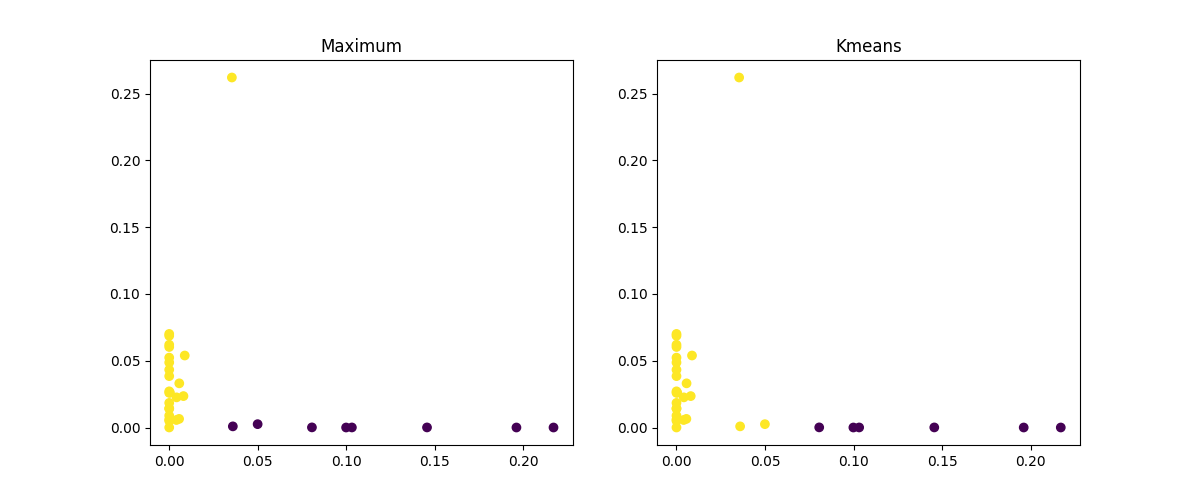
\includegraphics[width=\textwidth]{../plots/marko-bratu-clustering-1670776439.526882.png}
  \centering
  \end{figure}

  \[ A = \begin{pmatrix} 0.0007 & 0.9993 \\ 0.6302 & 0.3698 \end{pmatrix}  \] 

  From the $A$ matrix we may conclude that there's a very high probability to go into second
  state after the first one (vowel $\to$ consonant).

  \textit{Let's also analyse several other texts\ldots}

%%%%%%%%%%%%%%%%%%%%%%%%%%%%%%%%%%%%%%%%%%%%%%%%%%%%%%%%%%%%%%%%%%%%%%%%%%%%%%%%%%%%%%%%%%%%%%%%

  \textbf{Марко Вовчок. Інститутка.}


  \begin{center}
  \begin{tabular}{ | r | l | }
    \hline
    Parameter & Value \\
    \hline
    N & 2 \\
    \hline
    Epsilon (precision) & 2e-3 \\
    \hline
    Min iterations & 20 \\
    \hline
    $P^{(0)}$ distribution & evenly \\
    \hline
    $A^{(0)}$ distribution & normal \\
    \hline
    $B^{(0)}$ distribution & normal \\
    \hline
    Observation space size & 63715 \\
    \hline
  \end{tabular}
  \end{center}

  Converged after \textbf{144 iterations}.

  \textbf{[Clustering by maximum]}
  \begin{enumerate}
    \item 'е' 'у' 'і' 'и' 'ь' 'я' 'о' 'а' 'ф'
    \item ' ' 'т' 'г' 'ш' 'в' 'ч' 'н' 'к' 'л' 'ю' 'д' 'с' 'щ' 'й' 'р' 'б' 'з' 'ж'
 'м' 'ц' 'п' 'х' 'є' 'ї'
  \end{enumerate}

  \textbf{[Clustering by kmeans]}
  \begin{enumerate}
    \item 'е' 'у' 'і' 'и' 'о' 'а'
    \item ' ' 'т' 'г' 'ш' 'в' 'ч' 'н' 'к' 'л' 'ю' 'д' 'ь' 'с' 'я' 'щ' 'й' 'р' 'б'
 'з' 'ж' 'м' 'ц' 'п' 'х' 'є' 'ї' 'ф'
  \end{enumerate}

  The results are pretty the same except the presence of letter 'ф' in the first group
  while clustering by maximum.

  \begin{figure}[h]
    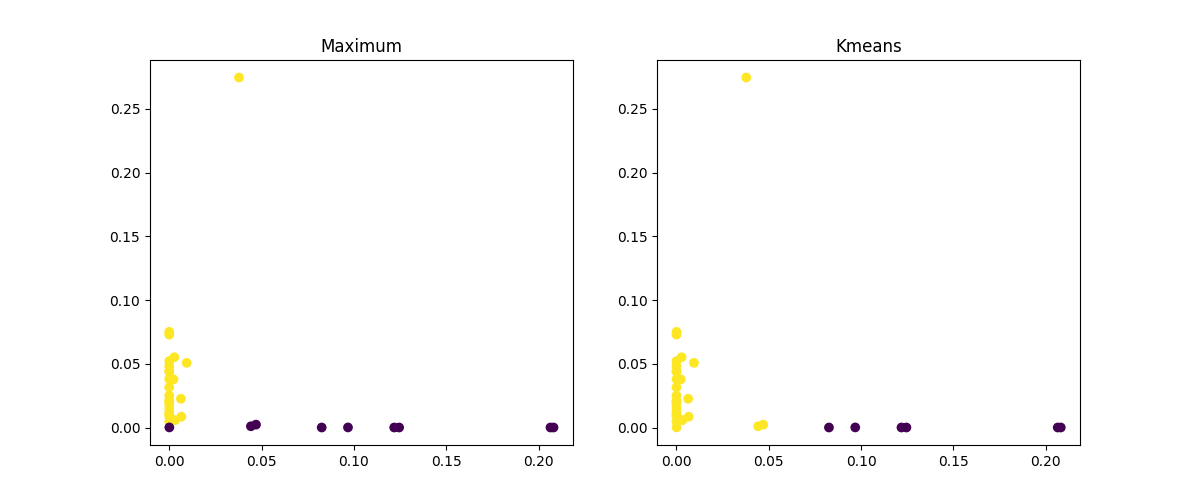
\includegraphics[width=\textwidth]{../plots/marko-instutytka-clustering-1670779387.3225758.png}
    \centering
  \end{figure}
	
  \[ A = \begin{pmatrix} 0.0011 & 0.9989 \\ 0.6147 & 0.3853 \end{pmatrix}  \] 



%%%%%%%%%%%%%%%%%%%%%%%%%%%%%%%%%%%%%%%%%%%%%%%%%%%%%%%%%%%%%%%%%%%%%%%%%%%%%%%%%%%%%%%%%%%%%%%%

  \subsection{Прихована марківська модель з трьома станами}

%%%%%%%%%%%%%%%%%%%%%%%%%%%%%%%%%%%%%%%%%%%%%%%%%%%%%%%%%%%%%%%%%%%%%%%%%%%%%%%%%%%%%%%%%%%%%%%%

  \textbf{Марко Вовчок. Інститутка.}

  \begin{center}
  \begin{tabular}{ | r | l | }
    \hline
    Parameter & Value \\
    \hline
    N & 3 \\
    \hline
    Epsilon (precision) & 2e-3 \\
    \hline
    Min iterations & 20 \\
    \hline
    $P^{(0)}$ distribution & evenly \\
    \hline
    $A^{(0)}$ distribution & normal \\
    \hline
    $B^{(0)}$ distribution & normal \\
    \hline
    Observation space size & 63715 \\
    \hline
  \end{tabular}
  \end{center}

  Converged after \textbf{271 iterations}.

  \textbf{[Clustering by maximum]}
  \begin{enumerate}
    \item 'т' 'г' 'в' 'ч' 'н' 'к' 'л' 'д' 'с' 'щ' 'р' 'б' 'ж' 'м' 'ц' 'п' 'х'
    \item 'е' 'у' 'і' 'и' 'ь' 'я' 'о' 'а'
    \item ' ' 'ш' 'ю' 'й' 'з' 'є' 'ї' 'ф'
  \end{enumerate}

  \textbf{[Clustering by kmeans]}
  \begin{enumerate}
    \item 'т' 'г' 'ш' 'в' 'ч' 'н' 'к' 'л' 'ю' 'д' 'ь' 'с' 'я' 'щ' 'й' 'р' 'б' 'з' 'ж' 'м' 'ц' 'п' 'х' 'є' 'ї' 'ф'
    \item 'е' 'у' 'і' 'и' 'о' 'а'
    \item ' '
  \end{enumerate}

  \begin{figure}[h]
    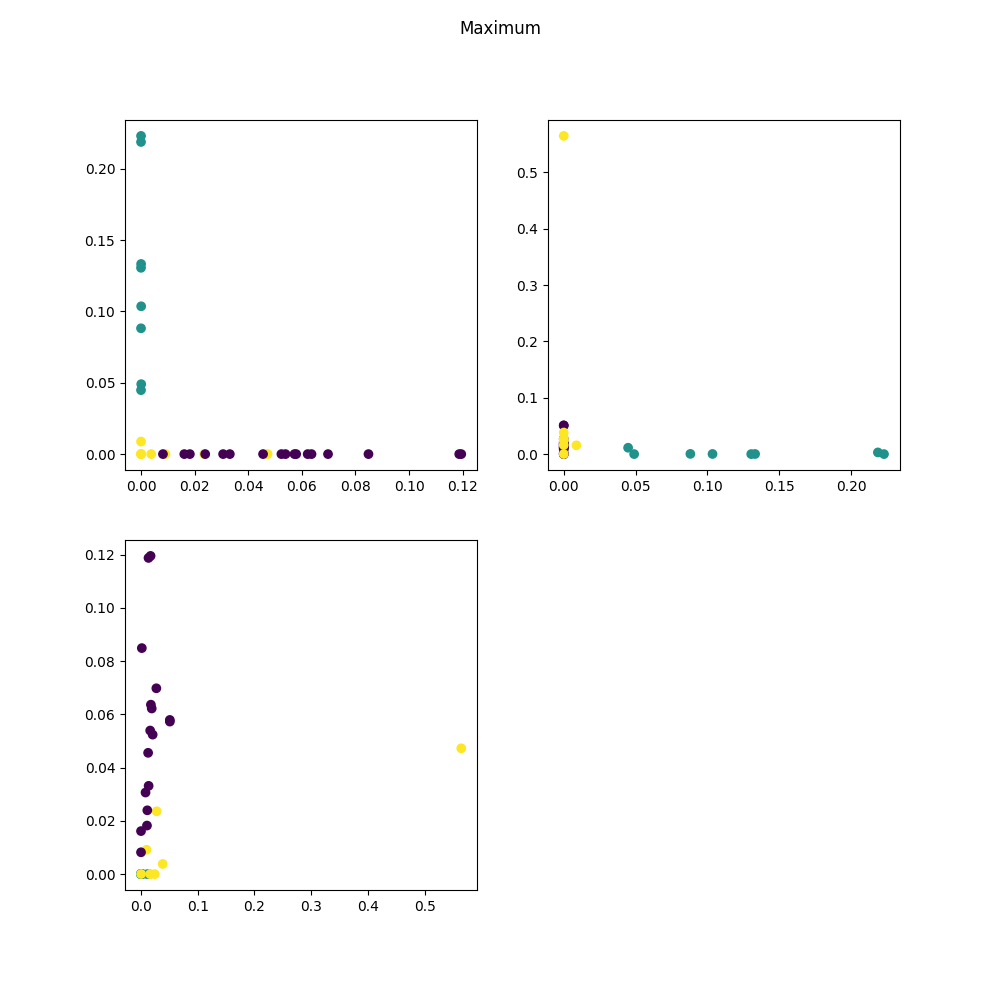
\includegraphics[width=\textwidth]{../plots/marko-instutytka-clustering-3-max-1670780571.6524851.png}
    \centering
    \caption{Clustering by maximum of HMM with 3 states trained on M.Vovchok 'Instytutka'}
  \end{figure}

  \begin{figure}[h]
    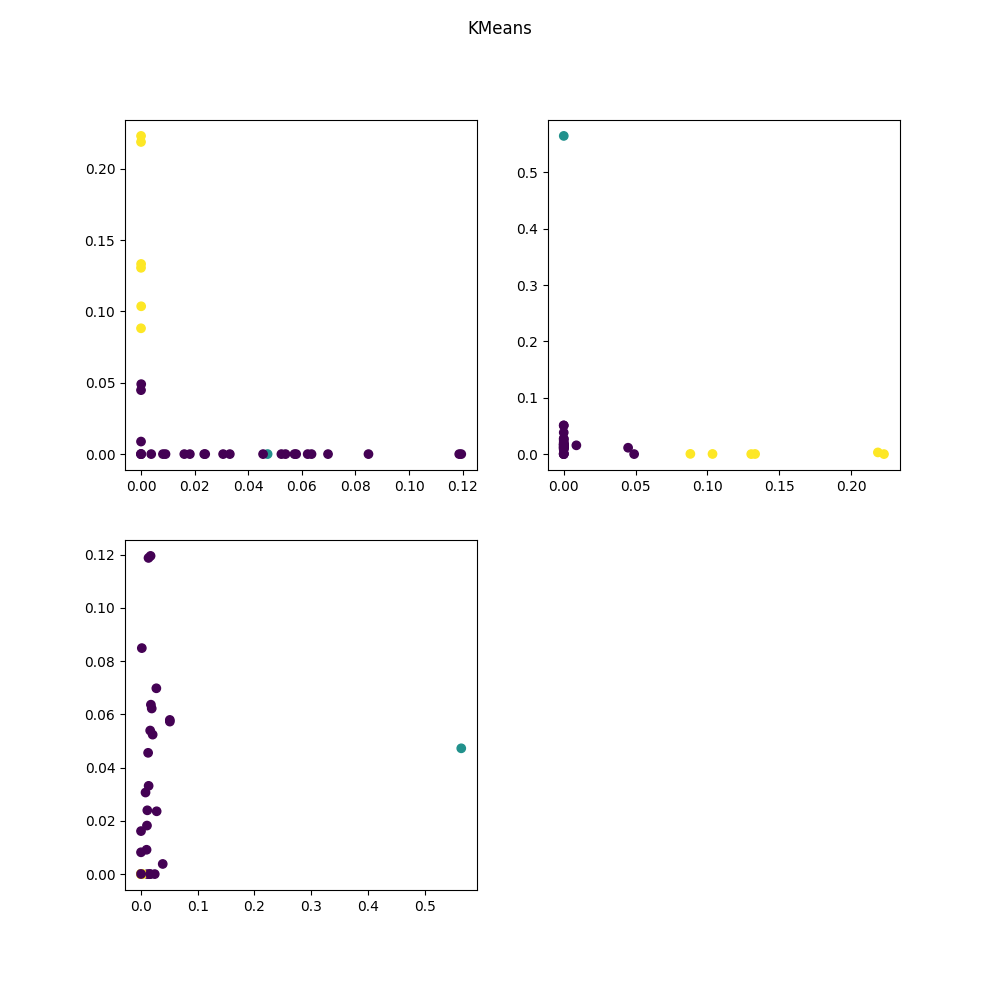
\includegraphics[width=\textwidth]{../plots/marko-instutytka-clustering-3-kmeans-1670780571.8452613.png}
    \centering
    \caption{Clustering by kmeans of HMM with 3 states trained on M.Vovchok 'Instytutka'}
  \end{figure}
	
  \[ A = \begin{pmatrix}
      0.0114 & 0.9886 & 0.0000 \\
      0.4226 & 0.0000 & 0.5774 \\
      0.6476 & 0.0420 & 0.3104
    \end{pmatrix}  \] 

  The third state cluster in a case of maximum clusterization may seem a weird one,
  but my opinion is that this class is a \textit{one-in-the-middle}. If we look at the
  $A$ matrix we can see that the transitions from the third class are all $> 0$.
  We cannot go into the third class from the first one (the consonants
  defined there).

  But the K-Means clustering method clearly defined a space in a separate class
  with vowels and consonants in a two different classes.

  \clearpage

%%%%%%%%%%%%%%%%%%%%%%%%%%%%%%%%%%%%%%%%%%%%%%%%%%%%%%%%%%%%%%%%%%%%%%%%%%%%%%%%%%%%%%%%%%%%%%%%

  \subsection{Прихована марківська модель з чотирма станами}

%%%%%%%%%%%%%%%%%%%%%%%%%%%%%%%%%%%%%%%%%%%%%%%%%%%%%%%%%%%%%%%%%%%%%%%%%%%%%%%%%%%%%%%%%%%%%%%%

  \textbf{Марко Вовчок. Інститутка.}

  \begin{center}
  \begin{tabular}{ | r | l | }
    \hline
    Parameter & Value \\
    \hline
    N & 4 \\
    \hline
    Epsilon (precision) & 1e-5 \\
    \hline
    Min iterations & 20 \\
    \hline
    $P^{(0)}$ distribution & normal \\
    \hline
    $A^{(0)}$ distribution & normal \\
    \hline
    $B^{(0)}$ distribution & normal \\
    \hline
    Observation space size & 63715 \\
    \hline
  \end{tabular}
  \end{center}

  Converged after \textbf{999 iterations}.

  \textbf{[Clustering by maximum]}
  \begin{enumerate}
    \item 'е' 'у' 'і' 'и' 'ь' 'о' 'а'
    \item 'т' 'г' 'ш' 'ч' 'н' 'к' 'л' 'д' 'щ' 'р' 'б' 'ж' 'м' 'ц' 'п' 'х'
    \item ' ' 'ю' 'є'
    \item 'в' 'с' 'я' 'й' 'з' 'ї' 'ф'
  \end{enumerate}

  \textbf{[Clustering by kmeans]}
  \begin{enumerate}
    \item 'е' 'у' 'і' 'и' 'о' 'а'
    \item 'г' 'ш' 'ч' 'ю' 'ь' 'я' 'щ' 'й' 'з' 'ж' 'ц' 'х' 'є' 'ї' 'ф'
    \item ' '
    \item 'т' 'в' 'н' 'к' 'л' 'д' 'с' 'р' 'б' 'м' 'п'
  \end{enumerate}

  \begin{figure}[h]
    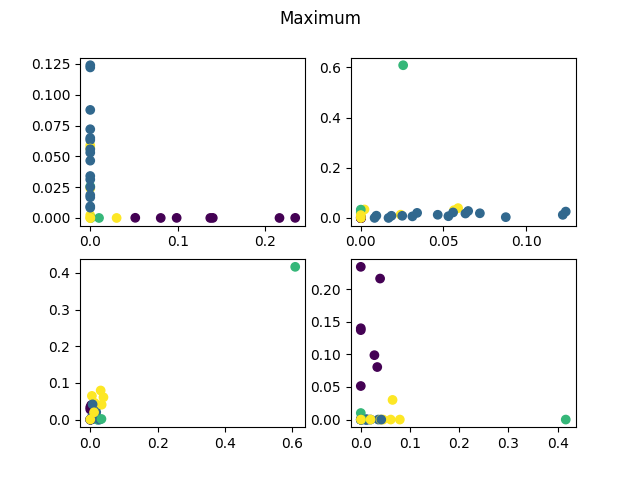
\includegraphics[width=\textwidth]{../plots/marko-instutytka-clustering-4-max-1670787549.9301946.png}
    \centering
    \caption{Clustering by maximum of HMM with 4 states trained on M.Vovchok 'Instytutka'}
  \end{figure}

  \begin{figure}[h]
    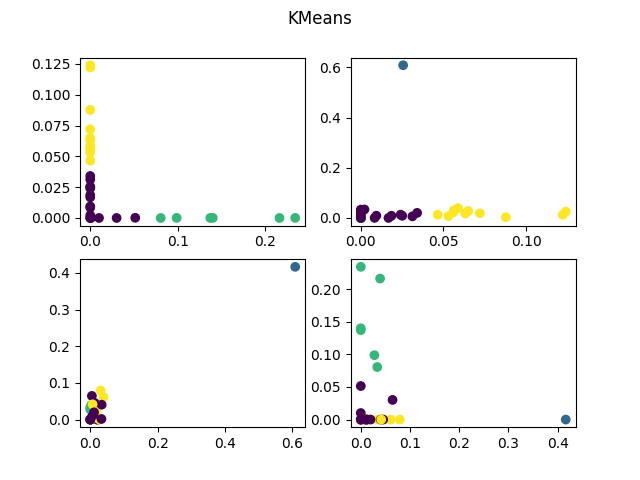
\includegraphics[width=\textwidth]{../plots/marko-instutytka-clustering-4-kmeans-1670787550.1034222.png}
    \centering
    \caption{Clustering by kmeans of HMM with 4 states trained on M.Vovchok 'Instytutka'}
  \end{figure}
	
  \[ A = \begin{pmatrix}
    0.0000 & 0.3996 & 0.5983 & 0.0021 \\
    0.9968 & 0.0009 & 0.0023 & 0.0000 \\
    0.0295 & 0.5959 & 0.0002 & 0.3744 \\
    0.0000 & 0.6115 & 0.0000 & 0.3885
  \end{pmatrix}  \] 

  \clearpage

%%%%%%%%%%%%%%%%%%%%%%%%%%%%%%%%%%%%%%%%%%%%%%%%%%%%%%%%%%%%%%%%%%%%%%%%%%%%%%%%%%%%%%%%%%%%%%%%

  \textbf{П. Куліш. Чорна Рада.}

  \begin{center}
  \begin{tabular}{ | r | l | }
    \hline
    Parameter & Value \\
    \hline
    N & 4 \\
    \hline
    Epsilon (precision) & 1e-2 \\
    \hline
    Min iterations & 35 \\
    \hline
    $P^{(0)}$ distribution & normal \\
    \hline
    $A^{(0)}$ distribution & normal \\
    \hline
    $B^{(0)}$ distribution & normal \\
    \hline
    Observation space size & 286868 \\
    \hline
  \end{tabular}
  \end{center}

  Converged after \textbf{141 iterations}.

  \textbf{[Clustering by maximum]}
  \begin{enumerate}
    \item ' '
    \item 'о' 'е' 'і' 'у' 'и' 'а' 'я' 'ь'
    \item 'в' 'к' 'є' 'ж' 'х' 'з' 'ш' 'м' 'й' 'ю' 'ї'
    \item 'п' 'с' 'н' 'р' 'д' 'б' 'л' 'г' 'т' 'ц' 'щ' 'ч' 'ґ' 'ф'
  \end{enumerate}

  \textbf{[Clustering by kmeans]}
  \begin{enumerate}
    \item ' '
    \item 'п' 'с' 'н' 'р' 'д' 'є' 'ж' 'х' 'б' 'я' 'л' 'ь' 'г' 'ш' 'т' 'ю' 'ц' 'ї'
 'щ' 'ч' 'ґ' 'ф'
    \item 'о' 'е' 'і' 'у' 'и' 'а'
    \item 'в' 'к' 'з' 'м' 'й'
  \end{enumerate}

  \begin{figure}[h]
    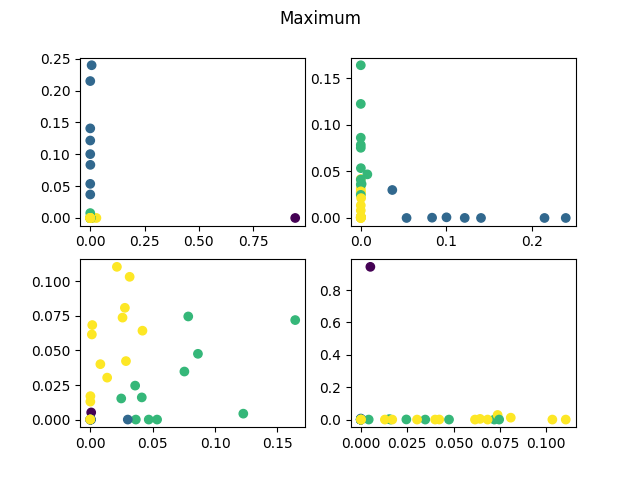
\includegraphics[width=\textwidth]{../plots/kylish-chorna-rada-clustering-4-max-1671021354.520232.png}
    \centering
    \caption{Clustering by maximum of HMM with 4 states trained on P.Kylish 'Chorna Rada'}
  \end{figure}

  \begin{figure}[h]
    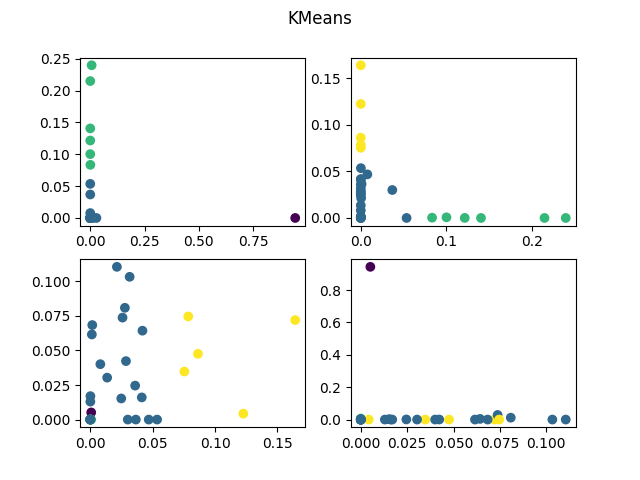
\includegraphics[width=\textwidth]{../plots/kylish-chorna-rada-clustering-4-kmeans-1671021354.8138266.png}
    \centering
    \caption{Clustering by kmeans of HMM with 4 states trained on P.Kylish 'Chorna Rada'}
  \end{figure}
	
  \[ A = \begin{pmatrix}
      0.0195 & 0.1296 & 0.0922 & 0.7588 \\
      0.3620 & 0.0000 & 0.1890 & 0.4490 \\
      0.6830 & 0.0000 & 0.0345 & 0.2826 \\
      0.0000 & 0.8853 & 0.0000 & 0.1147
  \end{pmatrix}  \] 

  \clearpage

%%%%%%%%%%%%%%%%%%%%%%%%%%%%%%%%%%%%%%%%%%%%%%%%%%%%%%%%%%%%%%%%%%%%%%%%%%%%%%%%%%%%%%%%%%%%%%%%


  \textbf{П. Куліш. Чорна Рада. (не враховуючи пробіли)}

  \begin{center}
  % \begin{tabular}{ | p{5cm} | p{1cm} | }
  \begin{tabular}{ | r | l | }
    \hline
    Parameter & Value \\
    \hline
    N & 4 \\
    \hline
    Epsilon (precision) & 1e-2 \\
    \hline
    Min iterations & 35 \\
    \hline
    $P^{(0)}$ distribution & normal \\
    \hline
    $A^{(0)}$ distribution & normal \\
    \hline
    $B^{(0)}$ distribution & normal \\
    \hline
    Observation space size & 234671 \\
    \hline
  \end{tabular}
  \end{center}

  Converged after \textbf{194 iterations}.

  \textbf{[Clustering by maximum]}
  \begin{enumerate}
    \item 'о' 'е' 'і' 'у' 'и' 'а'
    \item 'с' 'к' 'я' 'ь' 'ш' 'ґ'
    \item 'п' 'н' 'р' 'д' 'ж' 'б' 'л' 'г' 'м' 'т' 'ц' 'щ' 'ч' 'ф'
    \item 'в' 'є' 'х' 'з' 'й' 'ю' 'ї'
  \end{enumerate}

  \textbf{[Clustering by kmeans]}
  \begin{enumerate}
    \item 'с' 'ь'
    \item 'є' 'ж' 'х' 'б' 'я' 'з' 'г' 'ш' 'й' 'ю' 'ц' 'ї' 'щ' 'ч' 'ґ' 'ф'
 'щ' 'ч' 'ґ' 'ф'
    \item 'о' 'е' 'і' 'у' 'и' 'а'
    \item 'п' 'в' 'н' 'р' 'к' 'д' 'л' 'м' 'т'
  \end{enumerate}

  \begin{figure}[h]
    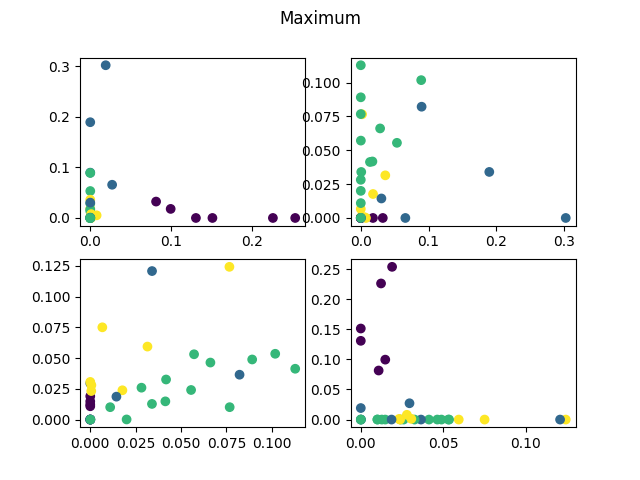
\includegraphics[width=\textwidth]{../plots/kylish-chorna-rada-without-spaces-clustering-4-max-1671021934.9575694.png}
    \centering
    \caption{Clustering by maximum of HMM with 4 states trained on P.Kylish 'Chorna Rada'}
  \end{figure}

  \begin{figure}[h]
    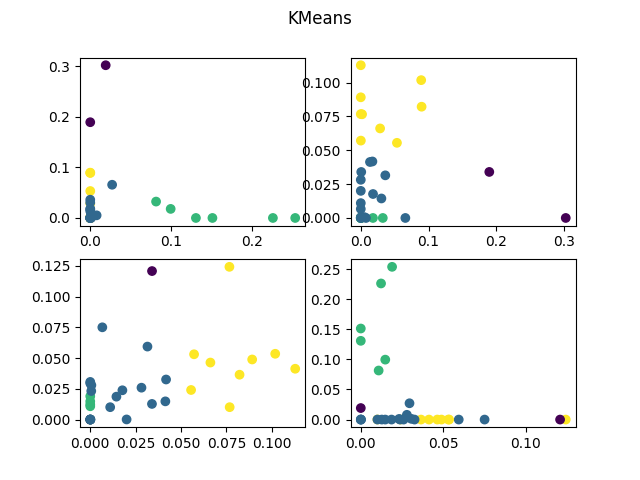
\includegraphics[width=\textwidth]{../plots/kylish-chorna-rada-without-spaces-clustering-4-kmeans-1671021935.735613.png}
    \centering
    \caption{Clustering by kmeans of HMM with 4 states trained on P.Kylish 'Chorna Rada'}
  \end{figure}
	
  \[ A = \begin{pmatrix}
      0.0195 & 0.1296 & 0.0922 & 0.7588 \\
      0.3620 & 0.0000 & 0.1890 & 0.4490 \\
      0.6830 & 0.0000 & 0.0345 & 0.2826 \\
      0.0000 & 0.8853 & 0.0000 & 0.1147
  \end{pmatrix}  \] 

  I think that the most clear results of HMM with 4 states
  are observed with the deletion of spaces.

  Here we can clearly see a set of sonorus letters
  \textit{'п' 'в' 'н' 'р' 'к' 'д' 'л' 'м' 'т'}
  in a case of the clustering by K-Means.

  Funny thing that the first class
  \textit{'с' 'ь'}
  is composed. Also useful to notice that this composition
  has a much higher frequence of 'сь'.

  \begin{center}
  \begin{tabular}{ | r | l | }
    \hline
    Чорна рада & 0.00663371306663692 \\
    \hline
    Дев'ять братів & 0.003378557422226933 \\
    \hline
    Кармелюк & 0.003376617962773829 \\
    \hline
  \end{tabular}
  \end{center}

  \clearpage

%%%%%%%%%%%%%%%%%%%%%%%%%%%%%%%%%%%%%%%%%%%%%%%%%%%%%%%%%%%%%%%%%%%%%%%%%%%%%%%%%%%%%%%%%%%%%%%%

  \section{Декодування зашифрованого тексту}

  As a encoding algorithm a simple alphabet shift was used.

  \textbf{Alphabet:} 'а', 'б', 'в', 'г', 'ґ', 'д', 'е', 'є', 'ж', 'з', 'и', 'і', 'ї', 'й', 'к', 'л', 'м', 'н', 'о', 'п', 'р', 'с', 'т', 'у', 'ф', 'х', 'ц', 'ч', 'ш', 'щ', 'ь', 'ю', 'я

  \begin{lstlisting}[language=Python]
encoded = ''
l = len(alphabet)
for s in text:
  encoded += alphabet[(alphabet.index(s) + shift) % l]
return encoded
  \end{lstlisting}

  \textbf{Марко Вовчок. Шифрування та декодування на основі одного тексту}

  Використаємо текст \textbf{Кармелюк} Марка Вовчка: зашифруємо його та
  використаємо для побудови параметрів для дешифрування.


  \begin{figure}[h]
    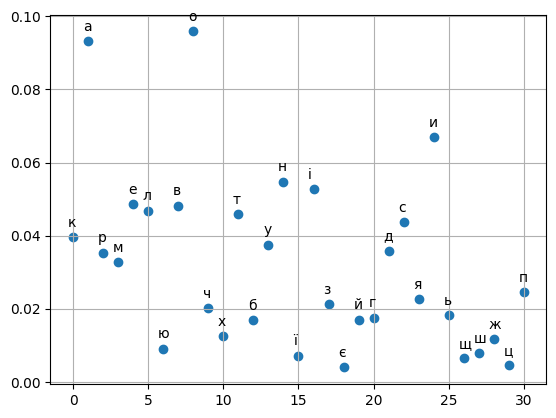
\includegraphics[width=12cm]{../text_frequencies/karmeluk.png}
    \centering
    \caption{Частоти літер твору \textit{Кармелюк}}
  \end{figure}

  Шифруємо текст зі зсувом 1:
  \textit{лбснємялгпгшплн...}

  Для побудови початкових параметрів для ПММ використаємо цей же твір.

  Матриця $A$ будується на біграмах з тексту, що будуть відповідати індексам
  літер з алфавіту $(i, j)$ відповідаючи рядкам та стовпцям матриці; обчислюємо
  кількість таких переходів літер на основі цих біграм, додаємо та нормуємо,
  додаючи перед цим до всіх значень у матриці $5$ для перетворення нульових
  ймовірностей у відносно близькі до нуля.

\begin{tabular}{lrrrrrrr}
   & 0        & 1        & 2        & 3        & 4        & 5        & \ldots \\
0  & 0.005726 & 0.019001 & 0.078605 & 0.019261 & 0.001301 & 0.045809 & \ldots\\
1  & 0.120192 & 0.009615 & 0.009615 & 0.006010 & 0.006010 & 0.006010 & \ldots\\
2  & 0.115031 & 0.015950 & 0.019333 & 0.014500 & 0.002417 & 0.025133 & \ldots\\
3  & 0.138211 & 0.006969 & 0.010453 & 0.005807 & 0.005807 & 0.009292 & \ldots\\
4  & 0.030303 & 0.030303 & 0.030303 & 0.030303 & 0.030303 & 0.030303 & \ldots\\
5  & 0.127054 & 0.007585 & 0.022756 & 0.003793 & 0.003161 & 0.008217 & \ldots\\
\vdots &\vdots &\vdots   &\vdots    &\vdots    &\vdots    &\vdots    &\ddots \\
30 & 0.012387 & 0.020270 & 0.037162 & 0.012387 & 0.005631 & 0.041667 & \ldots \\
31 & 0.024809 & 0.051527 & 0.040076 & 0.015267 & 0.009542 & 0.127863 & \ldots \\
32 & 0.013195 & 0.016023 & 0.063148 & 0.025448 & 0.004713 & 0.042413 & \ldots \\
\end{tabular}

За вектор $P$ візьмемо стаціонарний розподіл:
\[ \mu P = \mu \] 

\begin{align*}
  \mu = [ & 0.08554185 , 0.01852065 , 0.04605712 , 0.01916611 ,\\
               & 0.00367294 , 0.03521623 , 0.04643526 , 0.00719039 ,\\
               & 0.01397959 , 0.02239429 , 0.06246084 , 0.05001869 ,\\
               & 0.01001713 , 0.01865465 , 0.03848894 , 0.04485574 ,\\
               & 0.03250084 , 0.05180049 , 0.08790287 , 0.02526563 ,\\
               & 0.03470422 , 0.0420283 , 0.0440098 , 0.03663937 ,\\
               & 0.00367294 , 0.0146474 , 0.00770207 , 0.02148163 \\
               & 0.01057371 , 0.00934949 , 0.01976749 , 0.01166478 , 0.02361854 ]
.\end{align*}

Навчаємо ПММ на перших 3000 символах зашифрованого тексту
по алгоритму Баума-Велша з 33 станами, точністю в $1e-2$ та мінімальною
кількістю ітерацій в $200$.

\begin{figure}[h]
  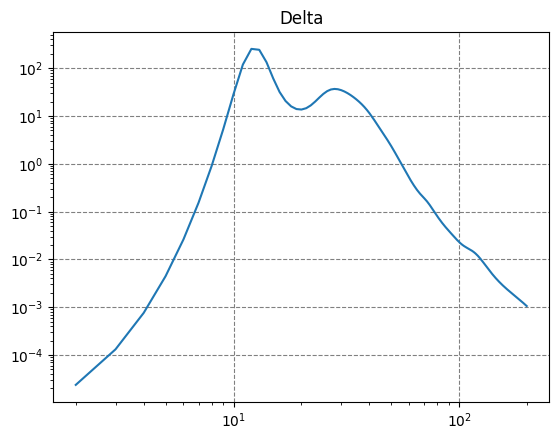
\includegraphics[width=10cm]{../plots/delta_karmeluk_karmeluk.png}
  \centering
  \caption{Еволюція дельти під час процедури навчання по параметрам текста Кармелюк на зашифрованому тексті Кармелюк}
\end{figure}

Отримана у результаті навчання матриця $B$:

\begin{tabular}{lrrrrrrrrrrrrrrrrrrrrrrrrrrrrrrrrr}
  & 0        & 1        & 2        & 3        & 4        & 5        & 6        & \ldots \\
а & 0.000000 & 0.000000 & 0.000000 & 0.000000 & 0.000000 & 0.000000 & 0.000000 & \ldots\\
б & 0.847381 & 0.000000 & 0.000000 & 0.000000 & 0.195377 & 0.000000 & 0.000000 & \ldots\\
в & 0.000000 & 0.837261 & 0.000000 & 0.000000 & 0.000000 & 0.000000 & 0.000000 & \ldots\\
г & 0.000000 & 0.000000 & 0.865880 & 0.000000 & 0.000000 & 0.000001 & 0.000000 & \ldots\\
ґ & 0.000000 & 0.114226 & 0.000000 & 0.815231 & 0.000000 & 0.000000 & 0.000000 & \ldots\\
д & 0.000000 & 0.000000 & 0.000000 & 0.000000 & 0.000000 & 0.000000 & 0.000000 & \ldots\\
е & 0.000000 & 0.048512 & 0.000000 & 0.000000 & 0.000000 & 0.771587 & 0.000000 & \ldots\\
є & 0.000000 & 0.000000 & 0.000000 & 0.000000 & 0.000000 & 0.000000 & 1.000000 & \ldots\\
ж & 0.000000 & 0.000000 & 0.000000 & 0.000000 & 0.000000 & 0.000000 & 0.000000 & \ldots\\
з & 0.000000 & 0.000000 & 0.000033 & 0.013084 & 0.000000 & 0.000268 & 0.000000 & \ldots\\
и & 0.000000 & 0.000000 & 0.000000 & 0.000000 & 0.000000 & 0.000000 & 0.000000 & \ldots\\
і & 0.031037 & 0.000000 & 0.000000 & 0.000000 & 0.000000 & 0.000000 & 0.000000 & \ldots\\
ї & 0.046833 & 0.000000 & 0.000000 & 0.000000 & 0.804481 & 0.000000 & 0.000000 & \ldots\\
й & 0.000000 & 0.000000 & 0.000000 & 0.000000 & 0.000000 & 0.000000 & 0.000000 & \ldots\\
к & 0.000000 & 0.000000 & 0.000000 & 0.034353 & 0.000000 & 0.000000 & 0.000000 & \ldots\\
л & 0.000000 & 0.000000 & 0.000000 & 0.000000 & 0.000000 & 0.000000 & 0.000000 & \ldots\\
м & 0.000000 & 0.000000 & 0.000000 & 0.137331 & 0.000000 & 0.000000 & 0.000000 & \ldots\\
н & 0.000000 & 0.000000 & 0.133100 & 0.000000 & 0.000000 & 0.000000 & 0.000000 & \ldots\\
о & 0.000000 & 0.000000 & 0.000000 & 0.000000 & 0.000000 & 0.054901 & 0.000000 & \ldots\\
п & 0.074706 & 0.000000 & 0.000000 & 0.000000 & 0.000142 & 0.000000 & 0.000000 & \ldots\\
р & 0.000000 & 0.000000 & 0.000986 & 0.000000 & 0.000000 & 0.000000 & 0.000000 & \ldots\\
с & 0.000000 & 0.000000 & 0.000000 & 0.000000 & 0.000000 & 0.000000 & 0.000000 & \ldots\\
т & 0.000000 & 0.000000 & 0.000000 & 0.000000 & 0.000000 & 0.169358 & 0.000000 & \ldots\\
\vdots \\
ю & 0.000000 & 0.000000 & 0.000000 & 0.000000 & 0.000000 & 0.000000 & 0.000000 & \ldots\\
я & 0.000000 & 0.000000 & 0.000000 & 0.000000 & 0.000000 & 0.000000 & 0.000000 & \ldots\\
\end{tabular}

У такому вигляді вона є транспонованою через технічні причини.
Але ми можемо побачити, певну залежність у цій матриці: літера 'а' кодується
літерою 'б', 'б' кодується 'в' і так далі. Тобто побачили шифр.

Прогнавши через алгоритм Вітербі отримуємо послідовність станів на цьому тексті.

Перші 200 символів розшифрованого текста:

\noindent\fbox{%
\parbox{\textwidth}{%
\textit{кармелюквовчокмаркохтобувавнаукраїніхтознаукраїнухтобувавізнаєтойнехайзгадає\\
  ахтонебувавінезнаєтойнехайсобіуявитьщотамскрізьбіліхатиувишневихсадкахівесною\\
  весноюламдужегарноякусісадочкизьцвітутьґусісоло\ldots}
}%
}

Порахувавши кількість вгаданих літер на всьому тексті отримуємо 98.01160110438461 \%.

\begin{figure}[h]
  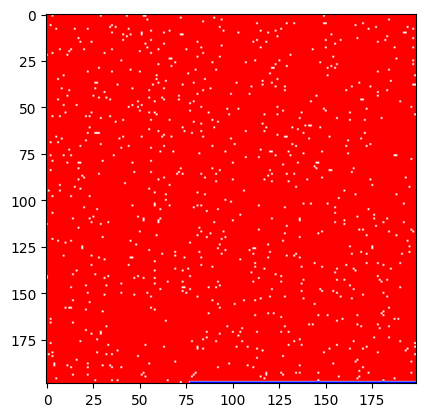
\includegraphics[width=10cm]{../plots/decoded_karmeluk_karmeluk.png}
  \centering
  \caption{Мапа правильного розкодування текста Кармелюк на основі текста Кармелюк}
\end{figure}

\textbf{Протестуємо весь процес на різних текстах.}

Нагадаю, що тексти мають таких авторів:

\begin{enumerate}
  \item Марко Вовчок. Дев'ять братів.
  \item Марко Вовчок. Інститутка.
  \item Марко Вовчок. Кармелюк.
  \item Марко Вовчок. Три долі.
  \item Пантелеймон Куліш. Чорна рада.
  \item Пантелеймон Куліш. Огненний змій
\end{enumerate}

\textbf{Інший текст для параметрів моделі.}

Візьмемо текст \textbf{Кармелюк} для шифрування та текст \textbf{Дев'ять братів}
як основу для параметрів моделі.

\begin{center}
  \begin{tabular}{| c | c | c | c | c | c | c |}
    \hline 
    & \multicolumn{6}{|c|}{Розміри тексту для навчання ПММ} \\
    \hline 
    & 1000 & 2000 & 3000 & 5000 & 8000 & 10000 \\
    \hline 
    Точність декодування & 88.49 & 92.07 & 0.60 & 0.04 & 97.95 & 97.67 \\
    \hline 
  \end{tabular}
\end{center}

Все ж можемо помітити наявність помилок у моделі на кроках у 3000 та 5000 розмірів
вибірки.

Та візьмемо інший текст: \textbf{Дев'ять братів} для шифрування та текст \textbf{Три долі}
як основу для параметрів моделі.

\begin{center}
  \begin{tabular}{| c | c | c | c | c | c | c |}
    \hline 
    & \multicolumn{6}{|c|}{Розміри тексту для навчання ПММ} \\
    \hline 
    & 1000 & 2000 & 3000 & 5000 & 8000 & 10000 \\
    \hline 
    Точність декодування & 0.25 & 89.90 & 0.20 & 93.30 & 0.20 & 0.20 \\
    \hline 
  \end{tabular}
\end{center}

Отже наша модель могла залишитися у якійсь точці локального мінімуму та видавати
поганий результат для задачі декодування. Але загалом зі збільшенням розміру вибірки
для навчання ПММ ми бачимо зростання точності декодування.

Як важливий крок для себе я б хотів додати, що спроба не залишатися на мові Python
та використати щось нове для себе дала чіткі плоди: я зміг не витрачати багато часу на
навчання ПММ (для прикладу на 33 станах та з вибіркою в 3000 символів для досягнення точності
в $1e-2$ знадобилося 200 ітерацій та 31 секунда часу, що дає 6.7 в середньому ітерацій на секунду,
а при взагалі простих умовах досягалося і 16-18 ітерацій на секунду) та використати його для збільшення розміру вибірки на задачі декодування.
Оптимізації у математиці беззаперечно дають добрий результат, як от
\textit{Forward-Backward procedure}, але й інструменти, які ми використовуємо, мають
відповідати нашим цілям.


% \begin{center}
% \begin{tabular}{| c | c | c | c | c | c | c |}
%   \hline
%   \% & \small{Дев'ять братів} & Інститутка & Чорна рада & Огненний змій \\
%   \hline
%   Дев'ять братів & 96.88 & & & \\
%   \hline \\
%   Інститутка \\
%   \hline \\
%   Чорна рада  \\
%   \hline \\
%   Огненний змій \\
%   \hline
% \end{tabular}
% \end{center}

\end{document}
